Our experiments share a common animation platform (our Experiment Setup) and a common Data Collection protocol.  Our experiments differ in presenting subjects with a range of Experimental Conditions.  All of the experiments described in this section together with the methods that we have chosen to analyze the data based on a private but approved pre-registration on \textit{aspredicted.org}. We will make the pre-registration public once the anonymity period ends.

\subsection{Experiment Setup}
Each animation shows a simulated robot producing two pointing gestures to specify a pick-and-place task.  Following the animation, viewers are asked whether a specific image represents a possible result of the specified task.

\noindent\textbf{Robotic Platforms}: The experiments were performed on two different robotic geometries, based on a \textit{Rethink Baxter}, and a \textit{Kuka IIWA14}.  The \textit{Baxter} is a dual-arm manipulator with two arms mounted on either side of a static torso. The experiments only move the right arm of the \textit{Baxter}. The \textit{Kuka} is consists of a single arm that is vertically mounted, i.e., points upward at the base. In the experiments the robots are shown with a singly fingered tooltip, where pointing gestures are modeled in terms of the outward ray coming out of the end-effector.

\noindent\textbf{Workspace Setup}: Objects are placed in front of the manipulators. In certain trials a table is placed in front of the robot as well, and the objects rest in stable configurations on top of the table. A pick-and-place task is provided specified in terms of the positions of one of the objects. 

\noindent\textbf{Objects}: The objects used in the study include small household items like mugs, saucers and boxes (cuboids), that are all placed in from on the robots.

\noindent\textbf{Motion Generation}: The end-effector of the manipulator is instructed to move to pre-specified waypoints, designed for the possibility of effective communication, that typically lie between the base of the manipulator and the object itself. Such waypoints fully specify both the position and orientation of the end-effector to satisfy \textit{pointing actions}. The motions are performed by solving \textit{Inverse-Kinematics} for the end-effector geometry and moving the manipulator along these waypoints using a robotic motion planning library \cite{littlefield2014extensible}. The motions were replayed on the model of the robot, and rendered in \textit{Blender}.

% \begin{figure}[t]
%     \centering
%     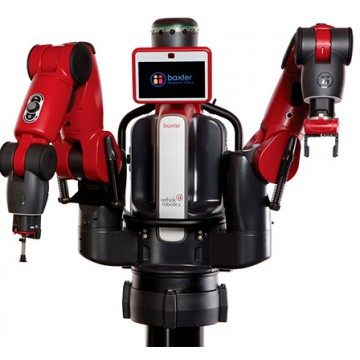
\includegraphics[width=0.23\textwidth]{baxter.jpg}
%     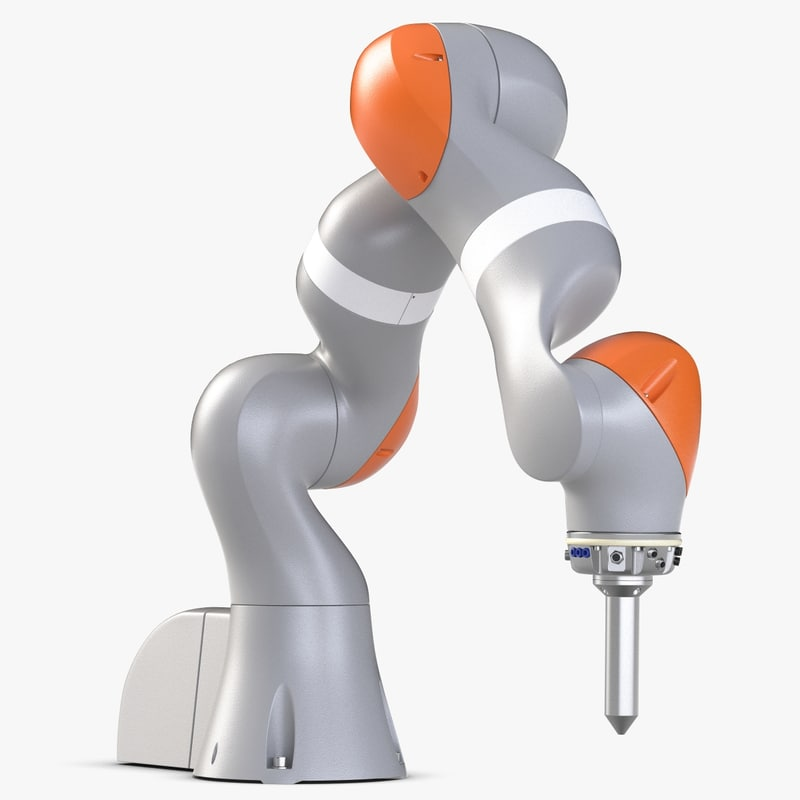
\includegraphics[width=0.23\textwidth]{kuka.jpg}
%     \caption{The robots used in the study are the \textit{Rethink Baxter}(left) and the \textit{Kuka IIWA14}(right)(<references>)}
%     \label{fig:robots}
% \end{figure}

\begin{figure}[th!]
    \centering
    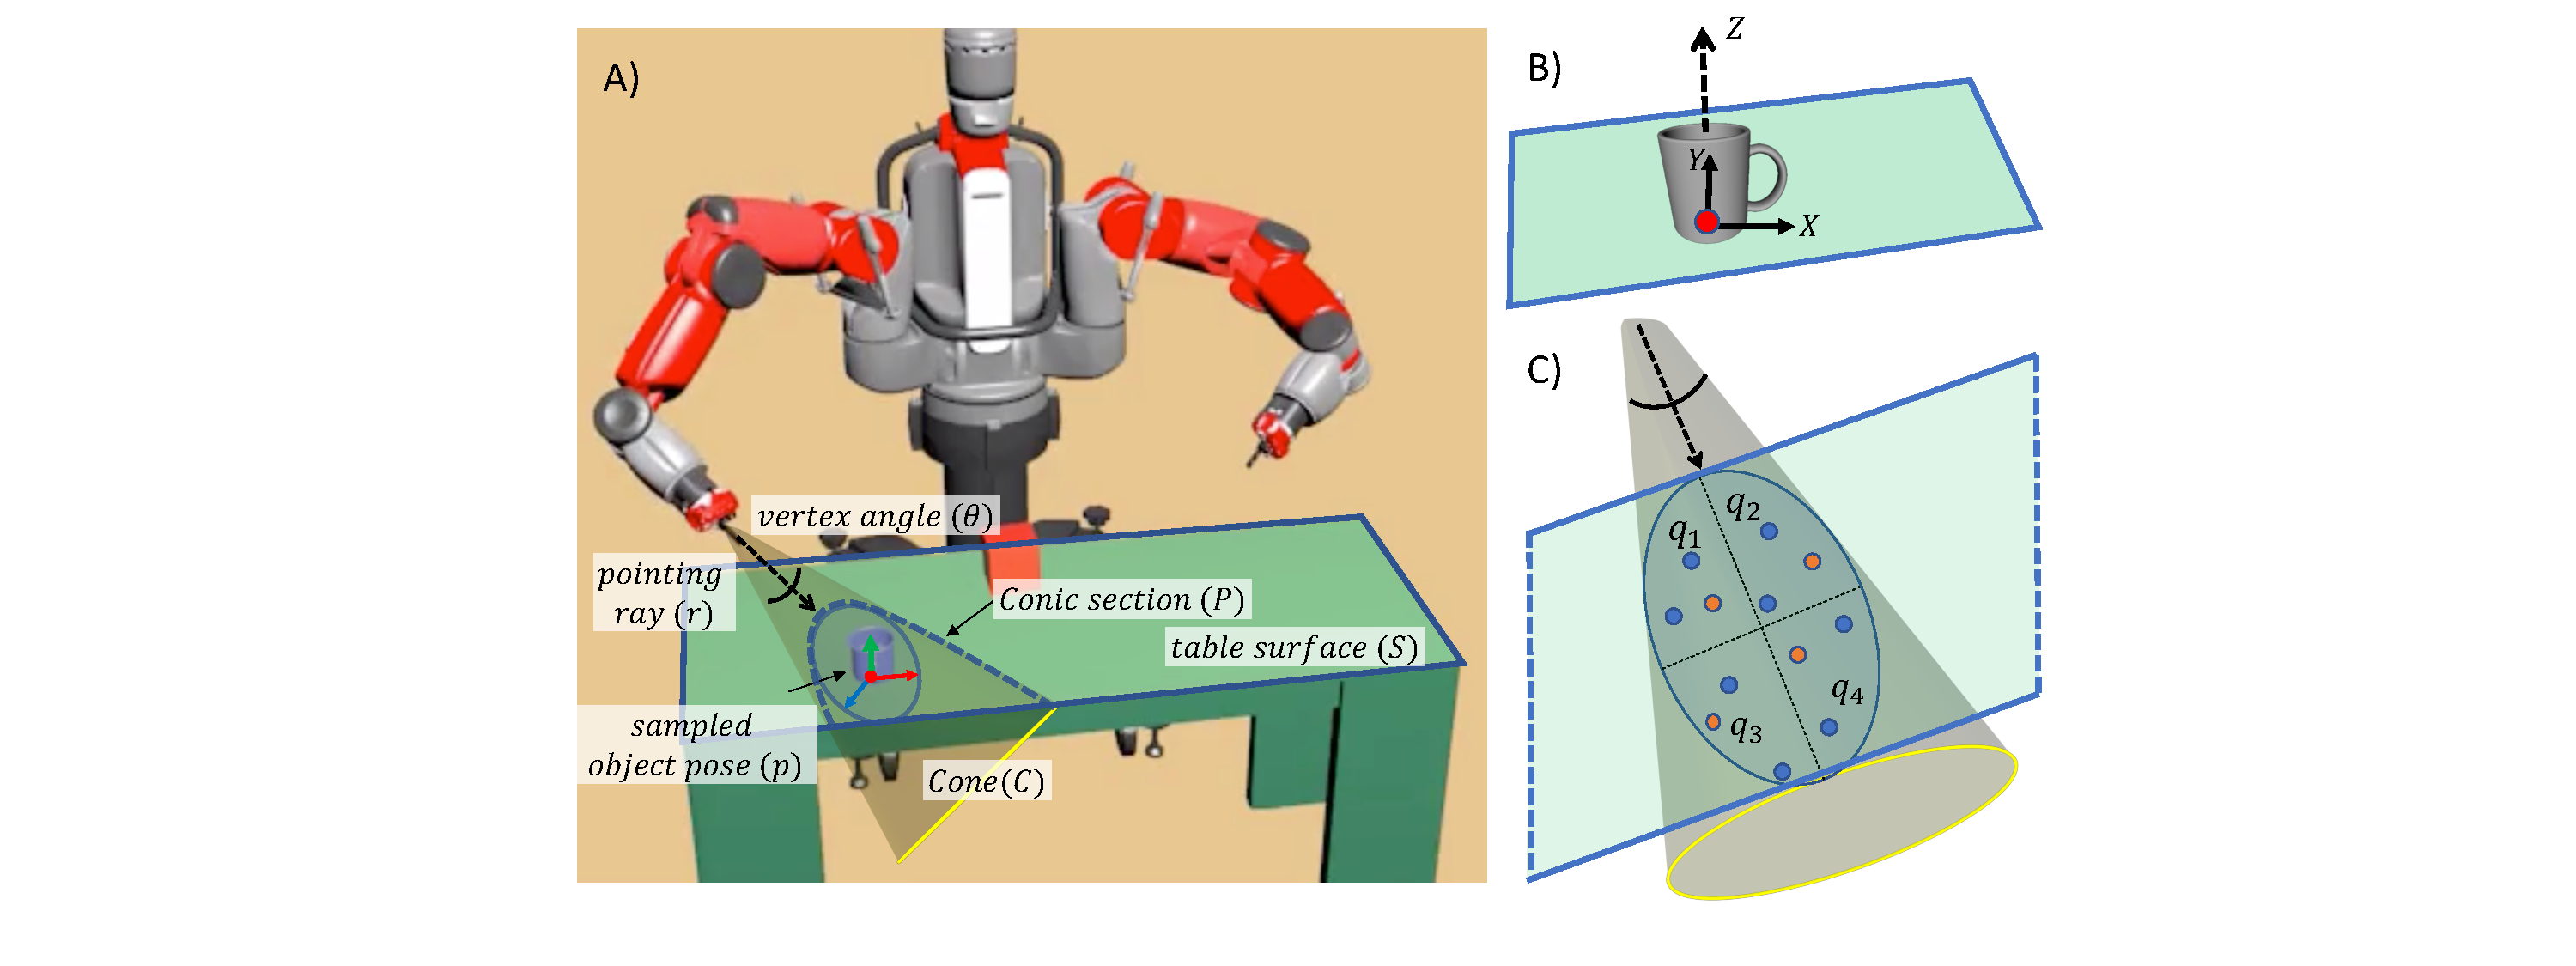
\includegraphics[width=0.5\textwidth]{pointing_diagram}
    \caption{(A) Workspace setup showing the pointing cone and the corresponding conic section on the table. (B) Shows the degrees-of-freedom considered for placement of the object on the table (C) Sampling policy to sample object poses within the conic section.}
    \label{fig:pointing}
\end{figure}

\begin{figure}[h!]
    \centering
    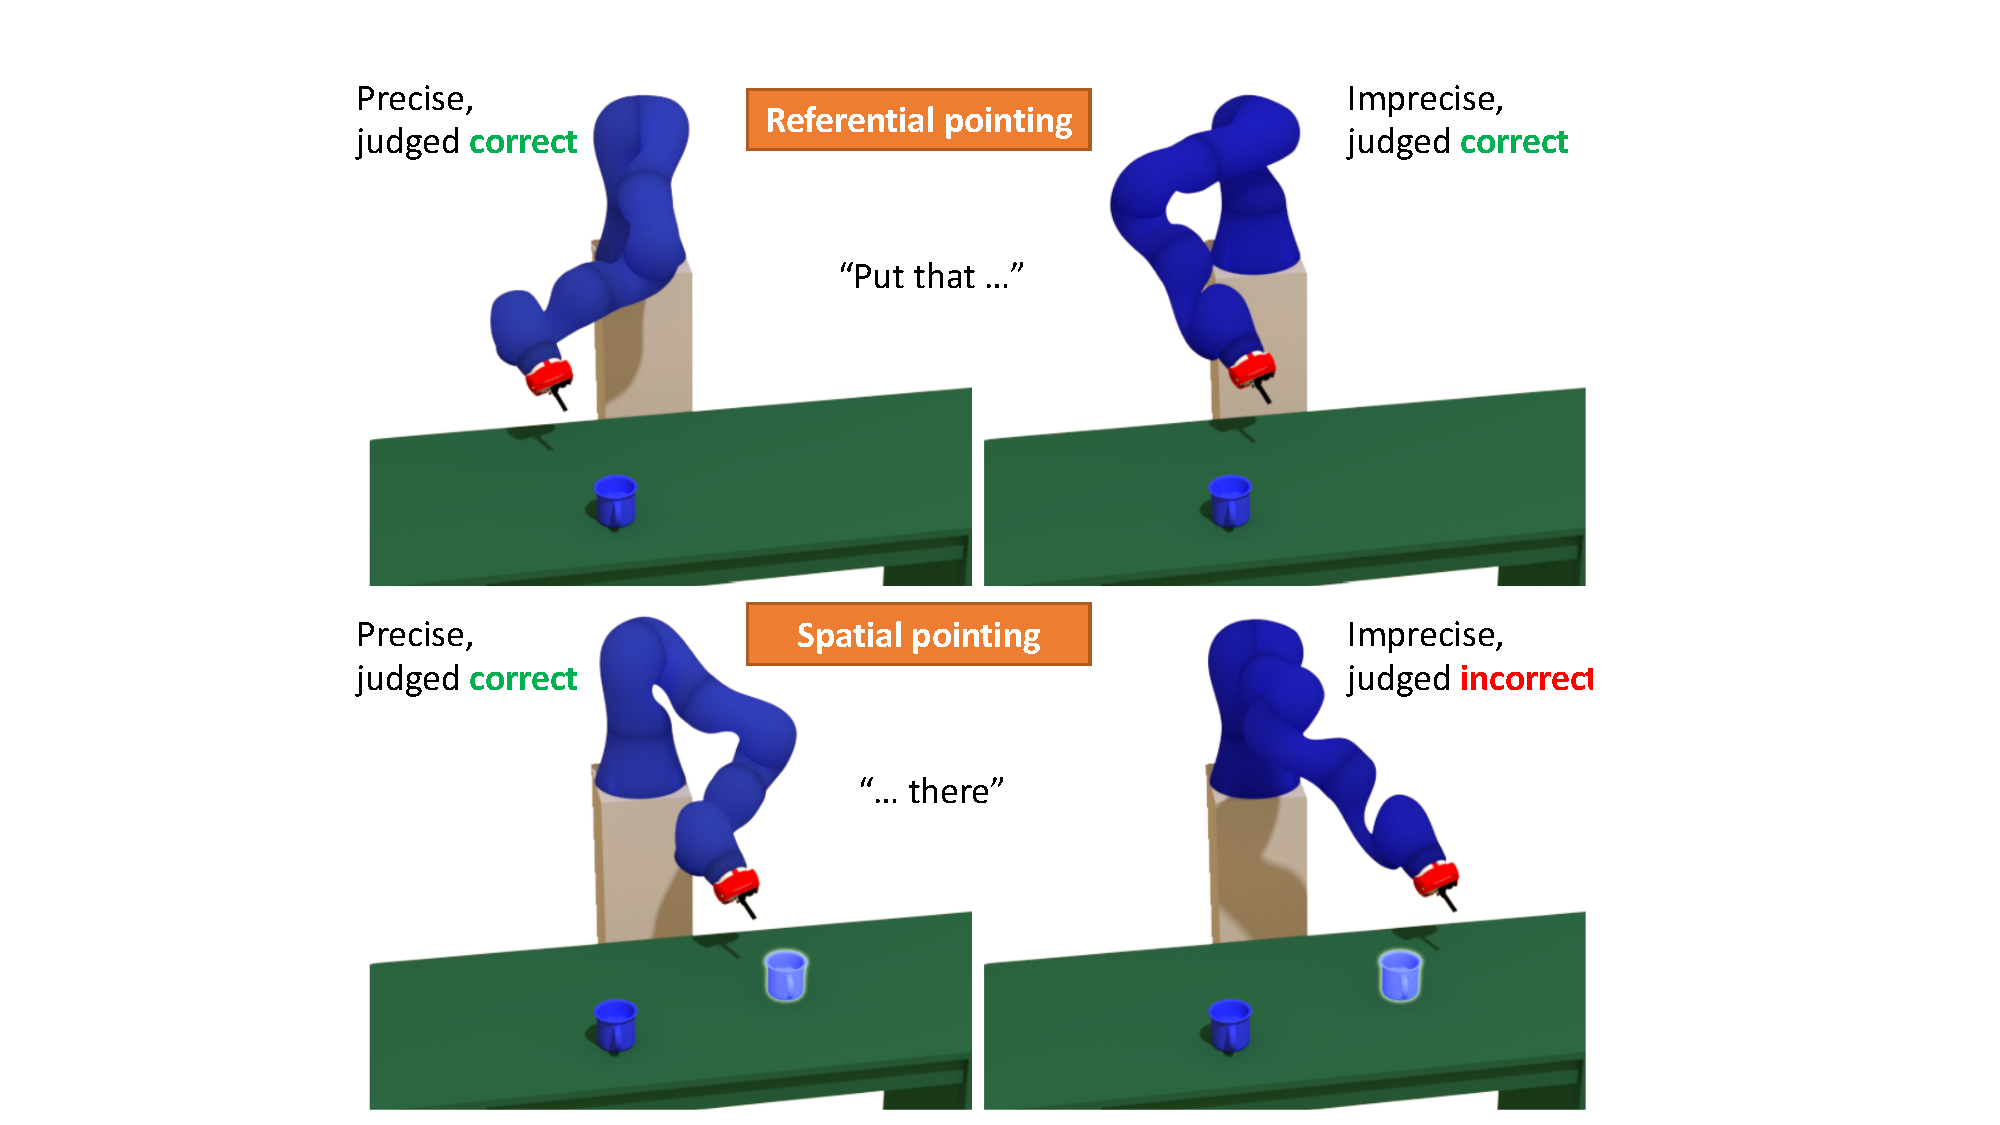
\includegraphics[width=0.48\textwidth]{spatial-referential.pdf}
    % 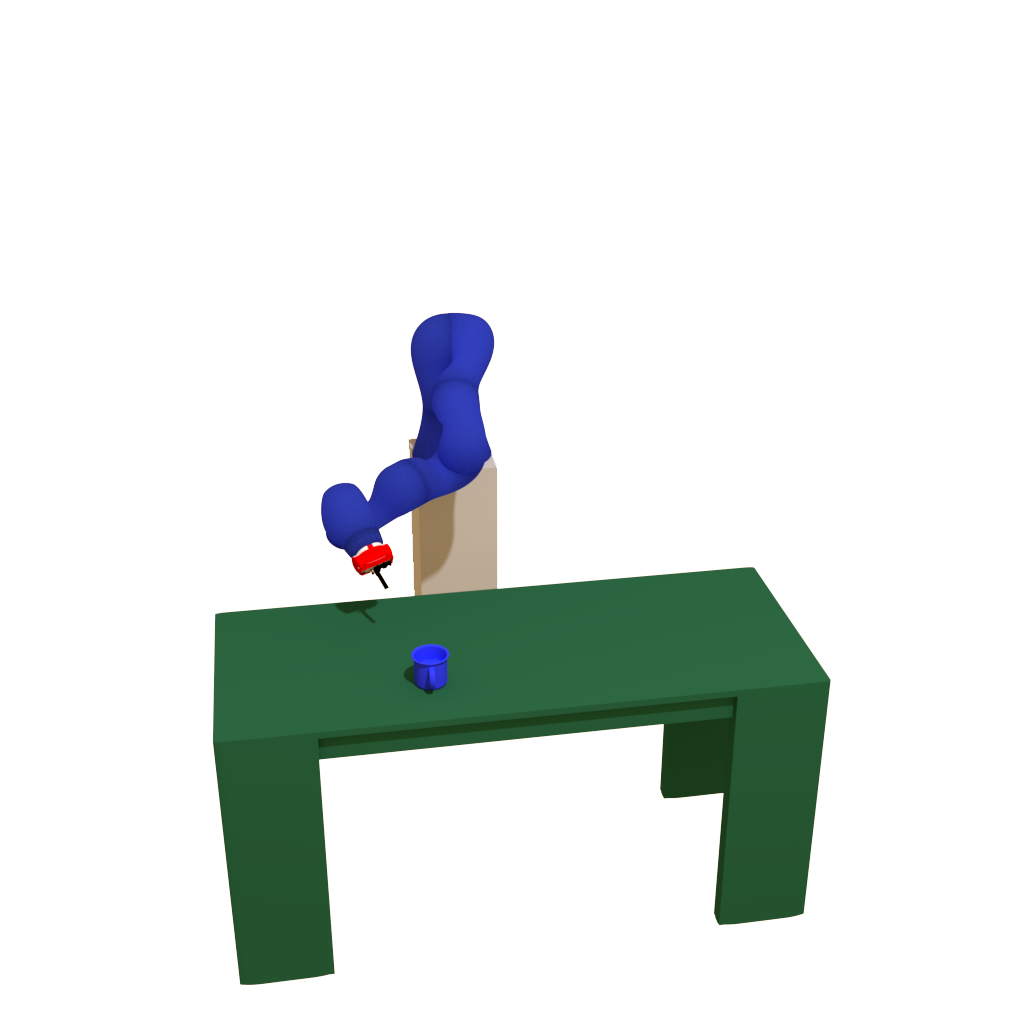
\includegraphics[width=0.23\textwidth, trim={3in 4in 4in 4in},clip]{figures/img11.png}
    % 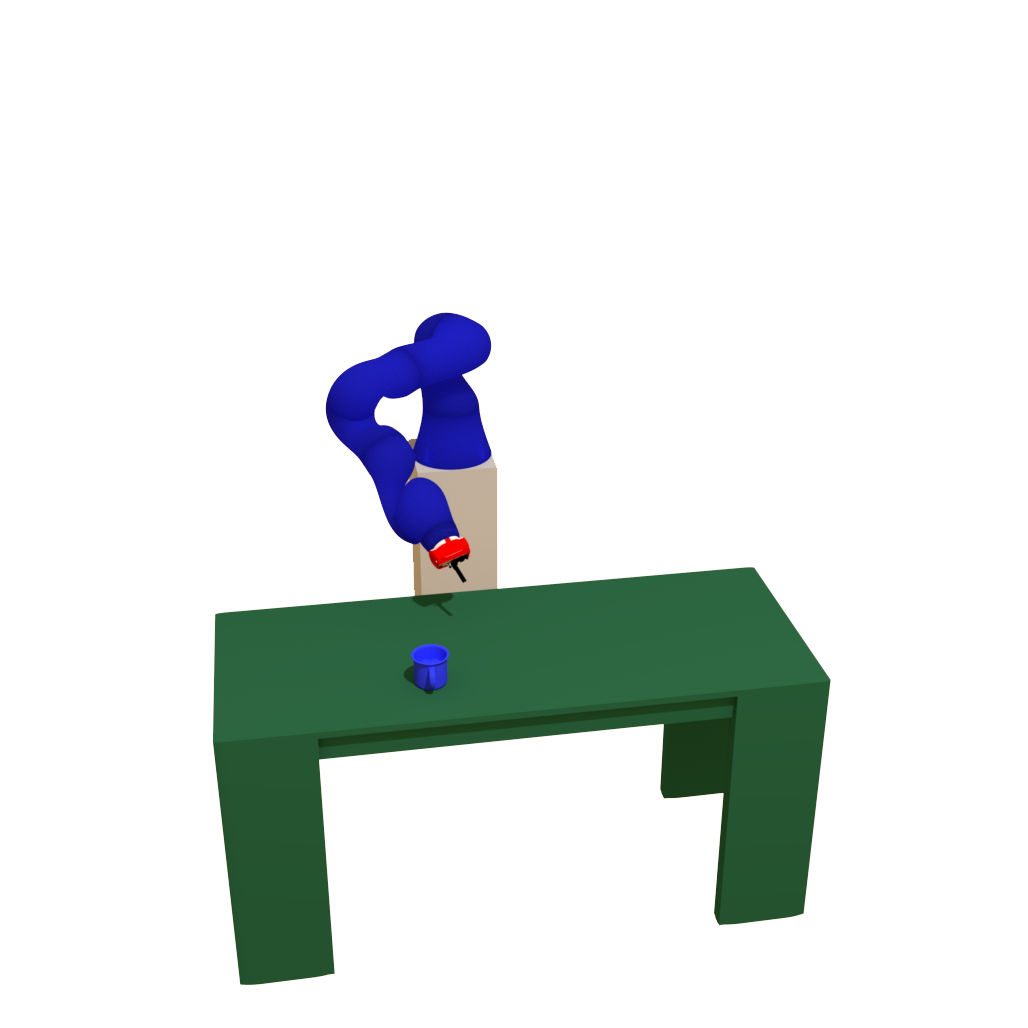
\includegraphics[width=0.23\textwidth, trim={3in 4in 4in 4in},clip]{figures/img21.png}
    % 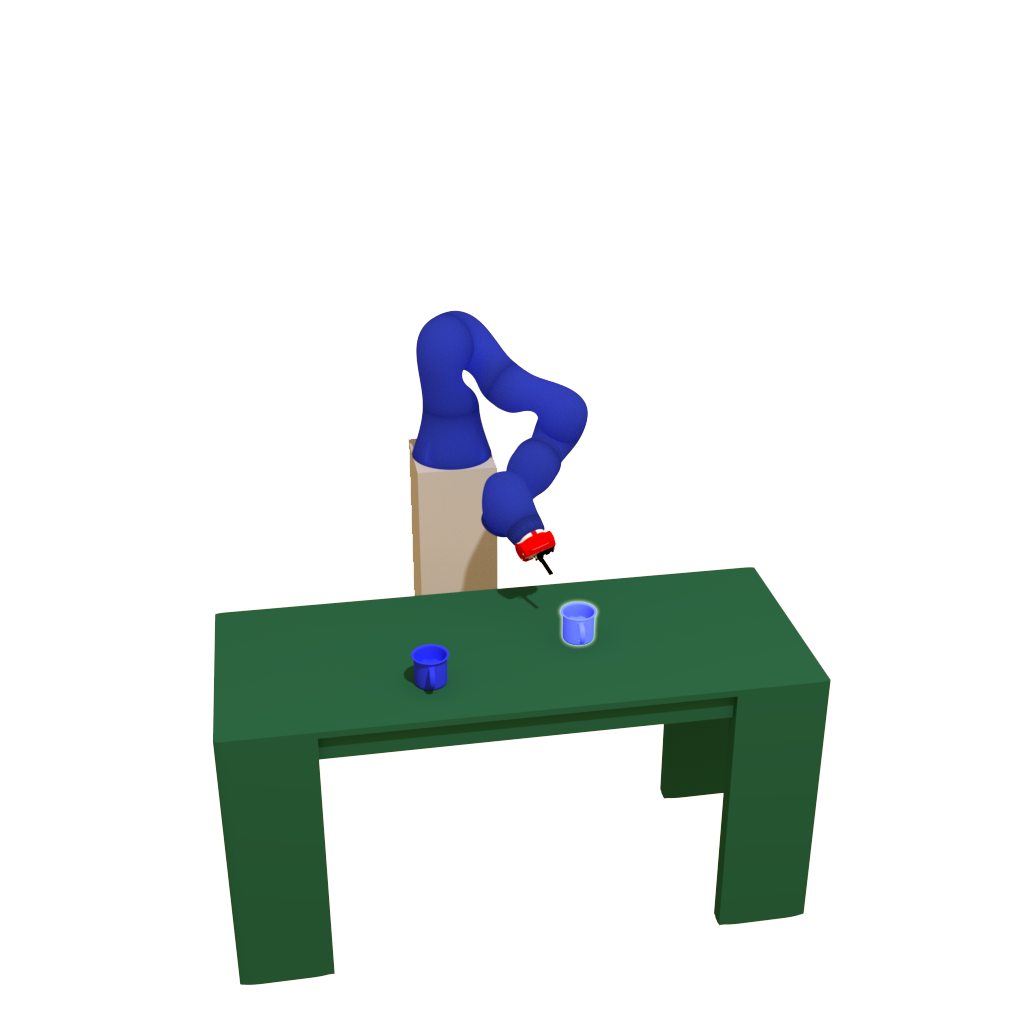
\includegraphics[width=0.23\textwidth, trim={3in 4in 4in 4in},clip]{figures/img12.png}
    % 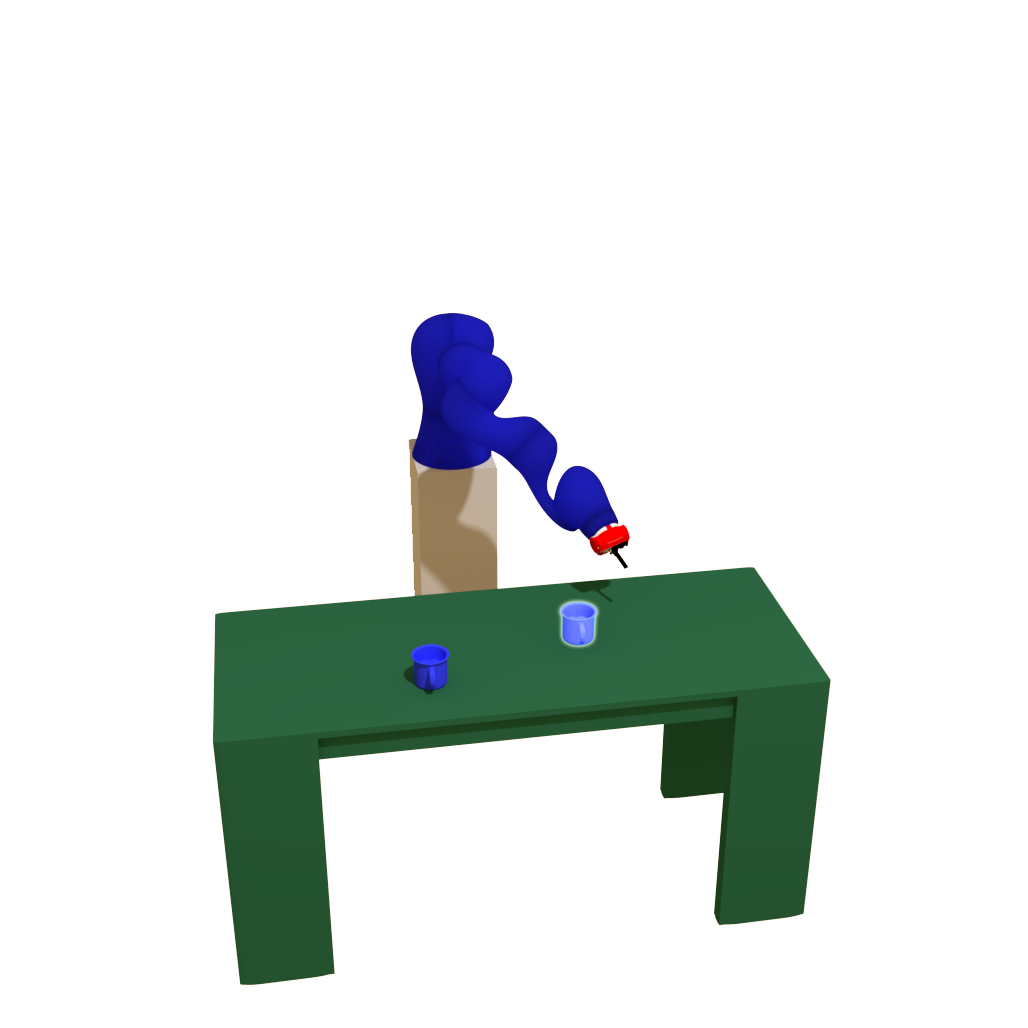
\includegraphics[width=0.23\textwidth, trim={3in 4in 4in 4in},clip]{figures/img22.png}
    \caption{The image shows the differences between referential (\textit{top}) and spacial pointing to the location of object placement (\textit{bottom}), demonstrated on a robotic manipulator, \textit{Kuka IIWA14}. An overlay of the object is shown at the placement location where spatial pointing needs to be directed.  Human subjects are more flexible with their interpretation of imprecise referential pointing than spatial.}
    \label{fig:spatial}
\end{figure}

\begin{figure}[h!]
    \centering
    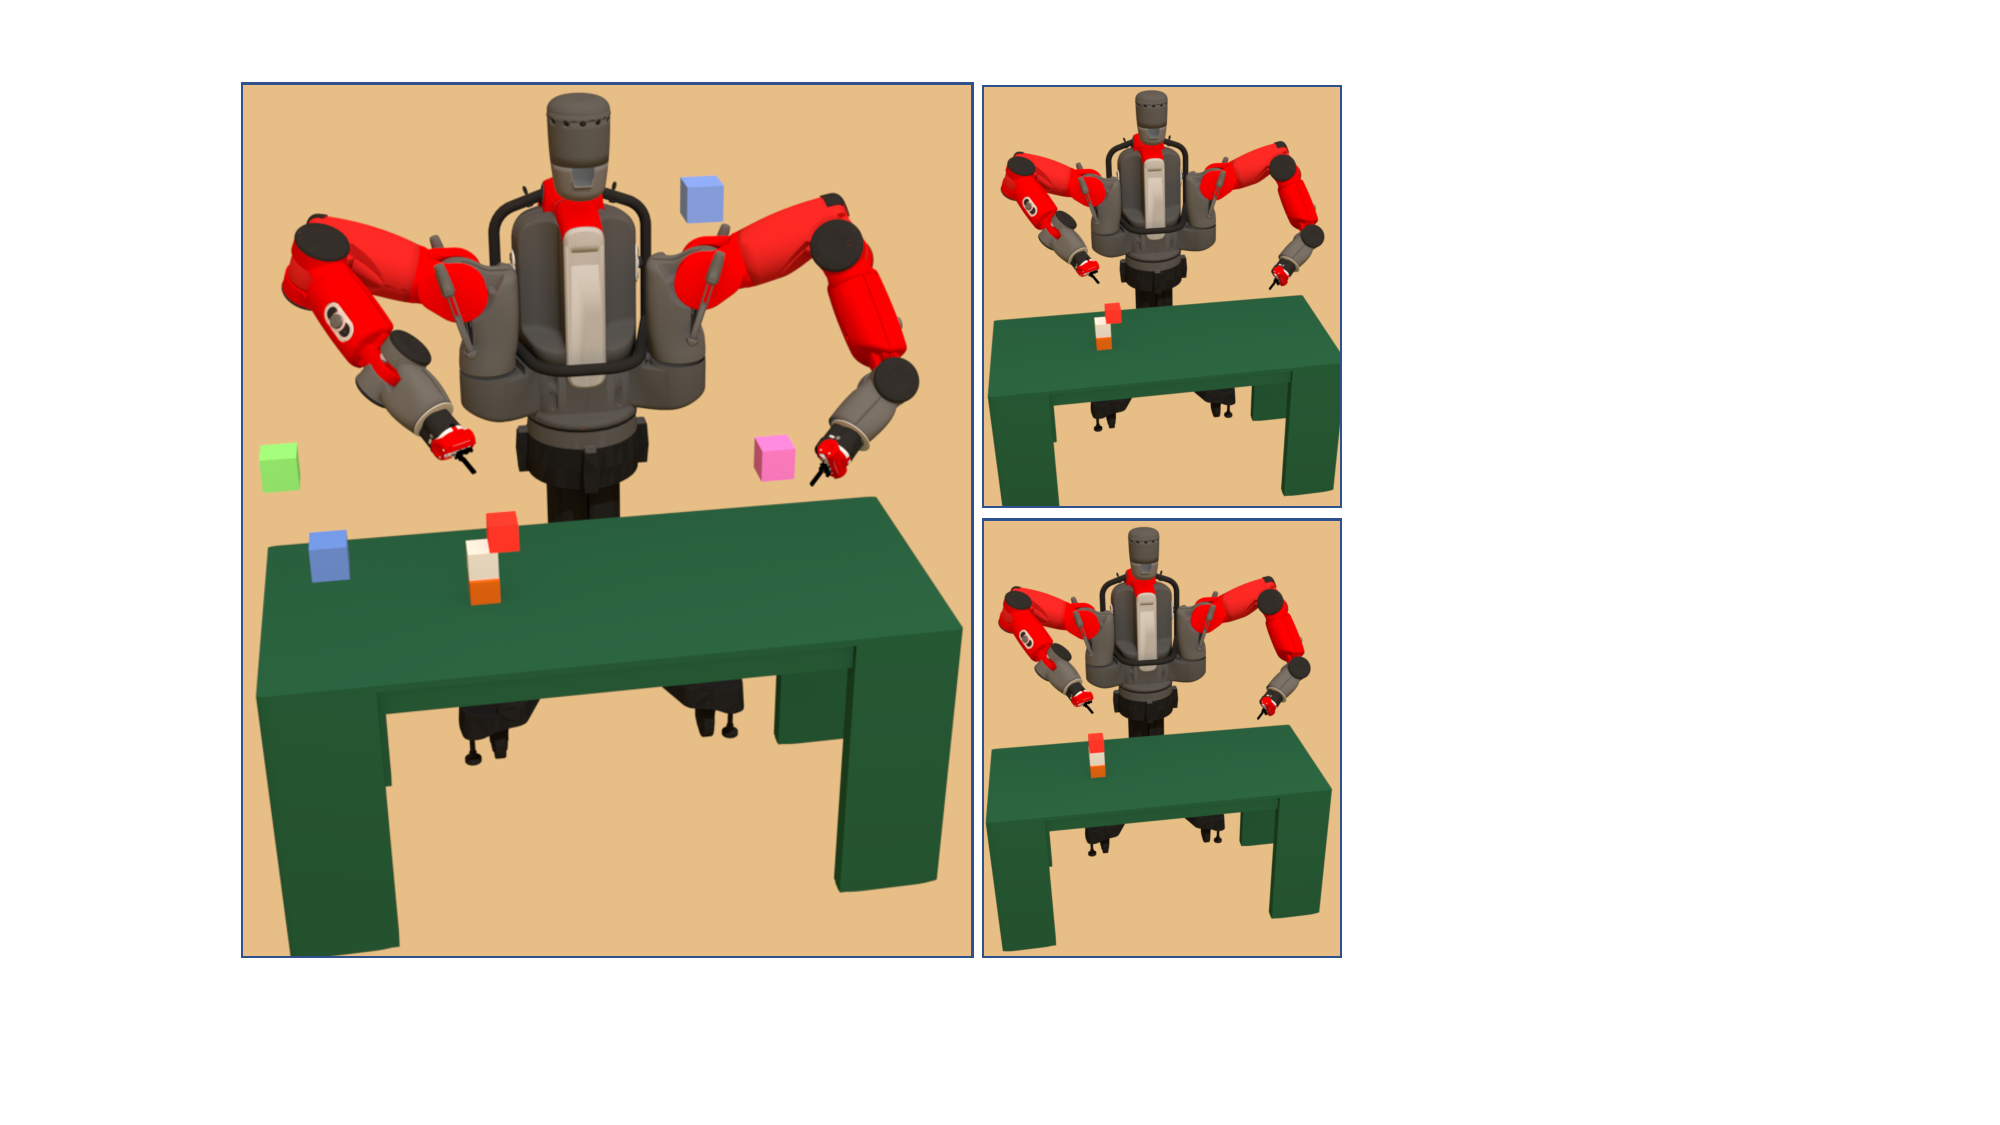
\includegraphics[width=0.45\textwidth]{natural.pdf}
    \caption{(Left) In an unnatural scene, a gesture pointing to an unstable position (edge of the stack) is deemed correct. (Right) In natural scenes, although the robot points to the edge of the stack, a physically realistic object position gets more user vote than the unstable position.}
    \label{fig:natural}
\end{figure}

% \noindent\textbf{Pointing Action Generation}: Pointing gesture is modeled by a cone $C(r, \theta)$ coming out of the pointing finger where $r$ represents the axis and $\theta$ represents the vertex angle of the cone. As illustrated in Fig~\ref{fig:pointing}, a robot is using it's finger to point to an object placed on a rest surface. For the scope of this study we assume that the rest surface is a plane represented by $S$. Thus the conic section formed on the surface of the table is given by $P=C \cap S$.

% To identify the geometry for the correct pointing gesture in different cases, $N$ object poses $p_i, i=1:N$ are sampled within the conic section $P$. While $p_i$ is the 6d pose for the object with translation $t \in R^3$ and orientation $R \in SO(3)$ only 3 degrees-of-freedom $(x, y, yaw)$ are varied for the experiments. By fixing the $z$ coordinate and the z-axis of rotation, it is ensured that the object rests in a physically stable configuration on the table.

% To sample $N$ poses, the largest eclipse that fits into the conic section $P$ is divided into 4 quadrants $q_1:q_4$ (See Figure~\ref{fig:pointing} (C)) . Within each quadrant $q_i$ the $N/4$ $(x,y)$ positions are sampled uniformly at random. For each placement $yaw$ is randomly sampled from the domain $(0, 2\pi)$. 

\noindent\textbf{Pointing Action Generation}: Potential pointing targets are placed using a cone $C(r, \theta)$, where $r$ represents the pointing ray and $\theta$ represents the vertex angle of the cone. As illustrated in Fig~\ref{fig:pointing}, the cone allows us to assess the possible divergence between the pointing ray and the actual location of potential target objects on the rest surface $S$. 

Given a pointing ray $r$, we assess the resolution of the pointing gesture by sampling $N$ object poses $p_i, i=1:N$ in $P=C(r, \theta) \cap S$---the intersection of the pointing cone with the rest surface.  While $p_i$ is the 6d pose for the object with translation $t \in R^3$ and orientation $R \in SO(3)$ only 2  degrees-of-freedom $(x, y)$ corresponding to $t$ are varied in the experiments. By fixing the $z$ coordinate for translation and restricting the z-axis of rotation to be perpendicular to $S$, it is ensured that the object rests in a physically stable configuration on the table.

The $N$ object poses are sampled by fitting an ellipse within $P$ and dividing the ellipse into 4 quadrants $q_1:q_4$ (See Figure~\ref{fig:pointing} (C)) . Within each quadrant $q_i$ the $N/4$ $(x,y)$ positions are sampled uniformly at random. For certain experiments additional samples are generated with an objective to increase coverage of samples within the ellipse by utilizing a dispersion measure.

% Malihe needs to check this.


\noindent\textbf{Speech}: Some experiments also included verbal cues with phrases like '\textit{Put that there}' along with the pointing actions. It was very important for the pointing actions and these verbal cues to be in synchronization. To fulfill this we generate the voice using Amazon Polly with text written in SSML format and make sure that peak of the gesture (the moment a gesture comes to a stop) is in alignment with the peak of each audio phrase in the accompanying speech. During the generation of the video itself we took note of the peak moments of the gestures and then manipulated the duration between peaks of the audio using SSML to match them with gesture peaks after analyzing the audio with the open-source tool PRAAT\footnote{www.praat.org}.

\subsection{Data Collection}

Data collection was performed in \textit{Amazon Mechanical Turk}.All subjects agreed to a consent form and were compensated at an estimated rate of \textit{USD 20} an hour. The subject-pool was restricted to non-colorblind US citizens. Subjects are presented a rendered video of the simulation where the robot performs one referential pointing action, and one spatial pointing action which amounts to it pointing to an object, and then to a final location. During these executions synchronized speech is included in some of the trials to provide verbal cues.

Then on the same page, subjects see the image that shows the result of the pointing action. They are asked whether the result is (a) correct, (b) incorrect, or (c) ambiguous.  

To test our hypothesis, we studied the interpretation of the two pointing behaviours in different contexts. Assuming our conjecture and a significance level of 0.05, a sample of 28 people in each condition is enough to detect our effect with a 95\% power.  Participants are asked to report judgments on the interpretation of the pointing action in each class.  Each participant undertakes two trials from each class.  The range of different cases are described below.  Overall, the data collection in this study involved over 7,290 responses to robot pointing actions.

\subsection{Experimental Conditions}

We used our experiment setup to generate videos and images from the simulation for a range of different conditions.

\paragraph{Referential vs Spatial}
In this condition, to reduce the chances of possible ambiguities, we place only one mug is on the table. The \textit{Baxter} robot points its right arm to the mug and then points to its final position, accompanied by a synchronized verbal cue, `\textit{Put that there.}'

% The final image then presents the accurate final position of the mug. Here, we vary the initial position of the mug that is we sample 8 random points from the three cones explained in section yyy. 

We keep the motion identical across all the trials in this method. 
We introduce a variability in the initial position of the mug by sampling $8$ random positions within conic sections subtending $45^{\circ} , 67.5^{\circ}, $ and $90^{\circ}$, on the surface of the table. New videos are generated for each such position of the mug.
This way we can measure how flexible subjects are to the variation of the initial location of the referent object. 

To test the effect for the spatial pointing action, we test similarly sampled positions around the final pointed location, and display these realizations of the mug as the result images to subjects, while the initial position of the mug is kept perfectly situated. 

 A red cube that is in the gesture space of the robot, and is about twice as big as the mug is placed on the other side of the table as a visual guide for the subjects to see how objects can be placed on the table. 

\noindent\textit{Effect of speech}: In order to test the effect of speech on the disparity between the kinds of pointing actions, a set of experiments were designed under the \textit{Referential vs Spatial} method with and without any speech. All subsequent methods will include verbal cues during their action execution. These cues are audible in the video.

\noindent\textit{Reverse Task}: One set of experiments are run for the pick-and-place task with the initial and final positions of the object flipped for the reverse task. This trial is designed to be identical the Referential vs Spatial trials, except for the direction. The motions are still executed on the \textit{Baxter's} right arm. 

\noindent\textit{Different Robotic Arm}:
In order to ensure that the results obtained in this study are not dependent on the choice of the robotic platform or its visual appearance, a second robot---a singly armed industrial \textit{Kuka} manipulator---is evaluated in the Referential vs Spatial study (shown in Figure~\ref{fig:spatial}).

\begin{figure}[t]
    % \vspace{-0.1in}
    \centering
    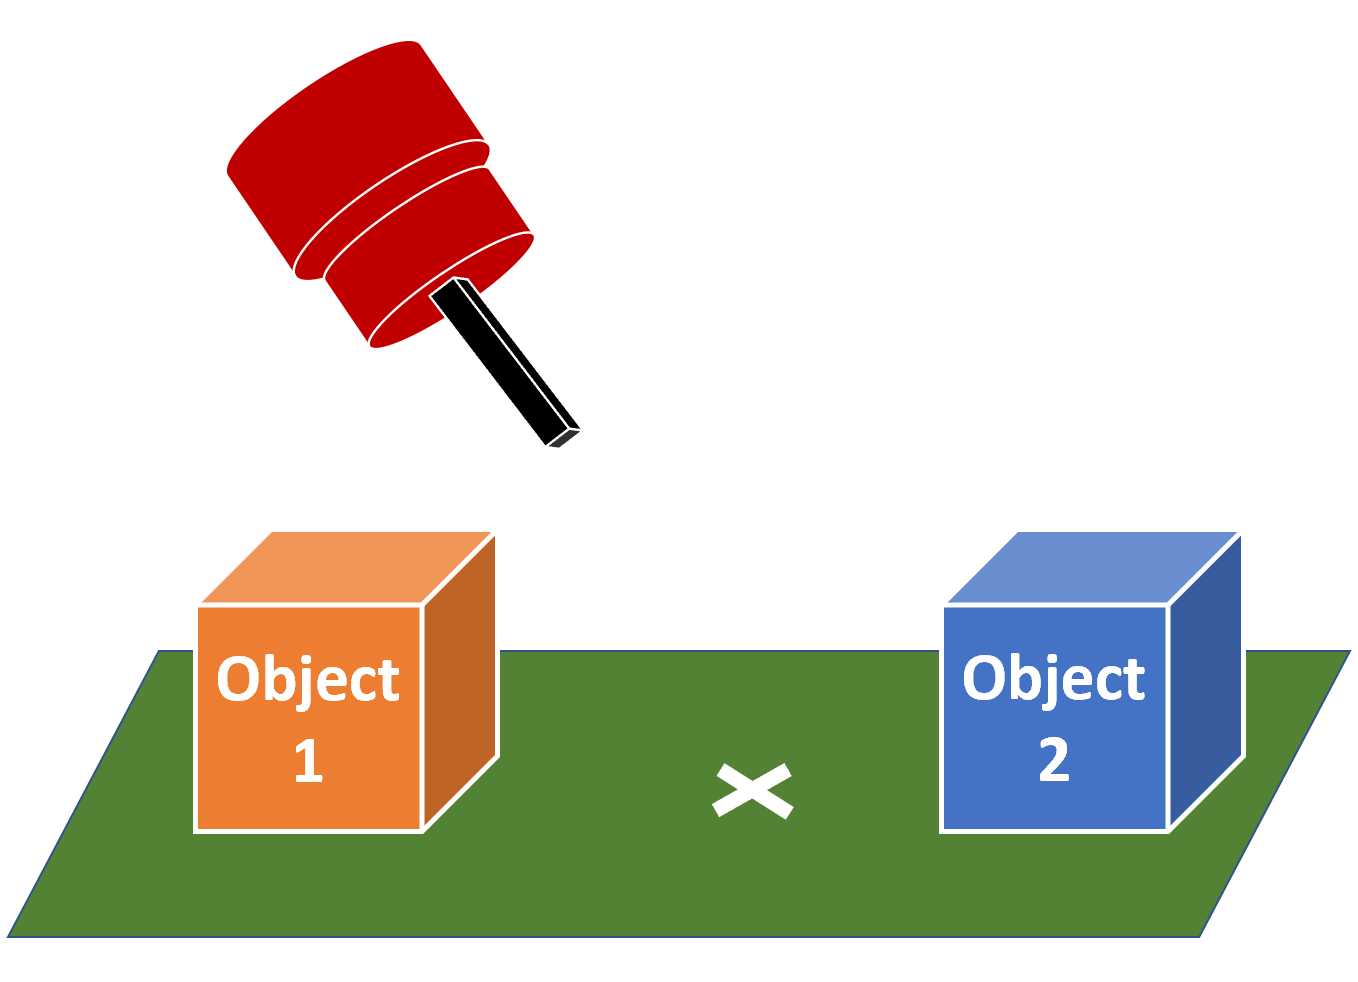
\includegraphics[width=0.3\textwidth]{figures/clutter_trial.png}
    \caption{A cluttered trial consists of collecting the response from a human subject when the position of the referential pointing action lies between two objects.}
    % \vspace{-0.3in}
    \label{fig:cluttered_trial}
\end{figure}

\paragraph{Cluttered Scene}
To study how the presence of other objects would change the behaviour of referential pointing, we examine the interpretation of the pointing actions when there are multiple objects on the tables. We start with a setup where there are 2 cups placed on the table (similar to the setup in Figure~\ref{fig:cluttered_trial}). One is a target cup placed at position $x_{object}$ and a distractor cup at position $x_{distractor}$. With the robot performing an initial pointing action to a position $x_{init}$ on the table. Both the objects are sampled around $x_{init}$ along the diametric line of the conic section arising from increasing cone angles of $45^\circ, 67.5^\circ, $ and $90^\circ$, where the separation of $x_{object}$, and $x_{distractor}$ is equal to the length of the diameter of the conic section, $D$. The objects are then positioned on the diametric line with a random offset between $[-\frac{D}{2}, \frac{D}{2}]$ around $x_{init}$ and along the line. This means that the objects are at various distances apart, and depending upon the offset, one of the objects is nearer to the pointing action. The setup induces that the nearer cup serves as the \textit{object}, and the farther one serves as the \textit{distractor}. The motions are performed on the \textit{Baxter's} right arm. The camera perspective in simulation is set to be facing into the pointing direction. The subjects in this trial are shown images of the instant of the referential pointing action.




\paragraph{Natural vs Unnatural scene}
In this experiment we study how the contextual and physical understanding of the world impacts the interpretation of pointing gestures. We generate a scenario for spatial pointing in which the right arm of the \textit{Baxter} points to a final placement position for the cuboidal object on top of a stack of cuboidal objects but towards the edge which makes it physically unstable. The final configurations of the object (Figure~\ref{fig:topedgetable}) shown to the users were a) object lying on top of the stack b) object in the unstable configuration towards the edge of the stack and c) object at the bottom of the stack towards one side. New videos are generated for each scenario along with verbal cues.

The pointing action, as well as the objects of interest stay the identical between the natural, and unnatural trials. The difference lies in other objects in the scene that could defy gravity and float in the unnatural trials. The subjects were given a text-based instruction at the beginning of an unnatural trial saying they were seeing a scene where "gravity does not exist". 



\paragraph{Different verbs}  
To test if the effect is specific to the verb \textit{put}, we designed a control condition where everything remained the same as the Referential vs Spatial trials except the verb \textit{put} which we replaced with \textit{place, move} and \textit{push}. Here again 30 data points for each sampled $x^*$

